\documentclass{article} 
\usepackage{amsmath} 
\usepackage{amssymb} 
\usepackage{amsthm} 
\usepackage[margin=0.2in]{geometry} 
\usepackage{hyperref} 
\usepackage{physics} 
\usepackage{tikz} 
\usepackage{mathtools}
\mathtoolsset{showonlyrefs} 
\theoremstyle{definition} 
\newtheorem{theorem}{Theorem}[section] 
\newtheorem{corollary}{Corollary}[theorem] 
\newtheorem{lemma}[theorem]{Lemma} 
\newtheorem{definition}{Definition}[section] 

\author{Connor Duncan}
\date{\today}

\title{notes-09-26-2019}
\begin{document}
\abstract{A single document copy of these notes, as well as a mirror of every note, can be found at \url{connorduncan.xyz/notes}}
\section{Indistinguishabe Particles} \begin{center} 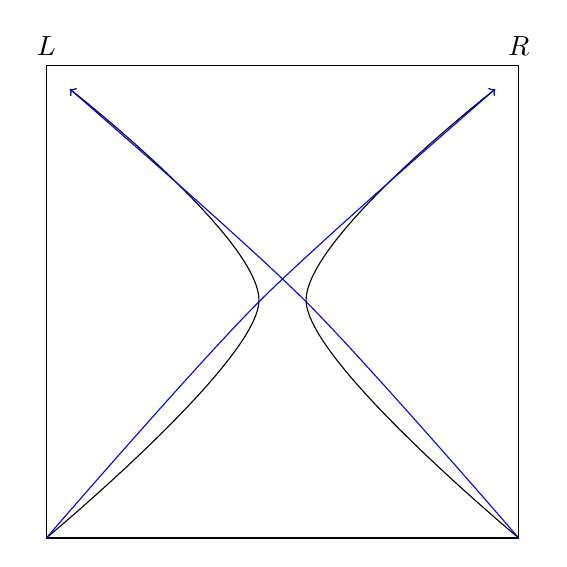
\begin{tikzpicture}[scale=3] \draw (-1,1) rectangle (1,-1); \node[anchor=south] (L) at (-1,1) {$L$}; \node[anchor=south] (R) at (1,1) {$R$}; \draw[->] plot [smooth] coordinates {(-1,-1) (-.1,0) (-.9,.9)}; \draw[->] plot [smooth] coordinates {(1,-1) (.1,0) (.9,.9)}; \draw[->,blue] plot [smooth] coordinates {(1,-1) (.1,0) (-.9,.9)}; \draw[->,blue] plot [smooth] coordinates {(-1,-1) (-.1,0) (.9,.9)}; \end{tikzpicture} \end{center} In this diagram, we cannot tell the difference between the black and blue particles, which means $\ket{L,R}$, $\ket{R,L}$ can't be the right states. It must be some superposition of these two states that gives us indistinguishability. Makes a lot of sense that it shouldl be eigensttates ofthe permutation operator. For the two particle system, these eigenstates are given by \begin{equation} \ket{\psi_\pm}=\frac{1}{\sqrt{2}}(\ket{LR}\pm\ket{RL}) \end{equation} \subsection{Bosons + Fermions} \begin{itemize} \item Bosons: Wavefunction must be symmetric under permutation. (Photons, Higgs Boson, Composite particles ($^4$He, Mesons) \item Fermions: Wavefunction is antisymmetric under permutation (Most fundamental particles, electrons protons neutrons, neutrinos, quarks) \end{itemize} Consider the case with two fermions. The only legal state of these is then \begin{equation} \frac{1}{\sqrt{2}}(\ket{\alpha_1,\alpha_2}-\ket{\alpha_2,\alpha_1}) \end{equation} if we let $\alpha_1=\alpha_2$ exactly, we immediately get the probability of finding two fermions in the same state as 0, which is just the \textbf{pauli exclusion principle}.
\end{document}
